\chapter{Methodology}

\paragraph{}
In this section, we describe our methodology for estimating behaviours of users in social media sites from observational data. Thanks to the literature we reviewed, we noticed that the interest and engagement are two crucial metrics for social media. These two values are dependant on many parameters which are not easy to determine. The user and the platform (Facebook, Twitter...) are the two main sources of variation. From the user perspective, their mood, stress and age \cite{f_youth_engagement} are factors modifying the two metrics. From the service side, the factors are well known from the companies, many engineers are focusing on developing better solutions for the user. These solutions are taking into consideration the content, the display, meta-data and are today more accurate thanks to Big Data (Facebook 100000 weight \cite{f_EdgeRank2}).\\
Due to three main reasons mentioned in the previous chapter which are privacy,content and technique, we based our experiment on Twitter. In this way, the content is normalised and the user is used to it because we embed the tweet: the design of each tweet is similar to the one on Twitter. In order to add fun, we picked the Tinder concept of binary classifications of girls and applied it to the tweets. This approach helped us to design a protocol based on tweets classification which differentiates the user interest and engagement.
Firstly, we give an overview of the methodology, explaining the test that we ran and the metrics used. Secondly, we introduce our Twitter dataset, composed of embedded tweets from user timelines. Final, we delve into the process itself.

\section{Big picture}

In order to measure our users behaviours, we decided to run A/B testing with two different B tests. It allows us 
to compare our dependent variables which are the number of likes and the time spent on a tweet. To be sure 
that we only keep in consideration the two dependent variables, a simple graphical design is used. This 
design is exactly like a PowerPoint document, where the content of each slide is an embedded tweet. The 
user has to decide for each slide, if he likes or dislikes a tweet by pressing one of two different keys on the 
keyboard. Based on this design, we create an A/B test with one initial experiment called "Calibration" (test A) 
and two other ones taking in input the time (test B1) and the numbers of likes (test B2). Because of the unique 
design, we are going to explain how we select the tweets for the calibration part and the two other tests. \\
\\
metrics: the time that a user is spending on a tweet, the decision (like / dislike) 

\begin{figure}[h] 
\centering 
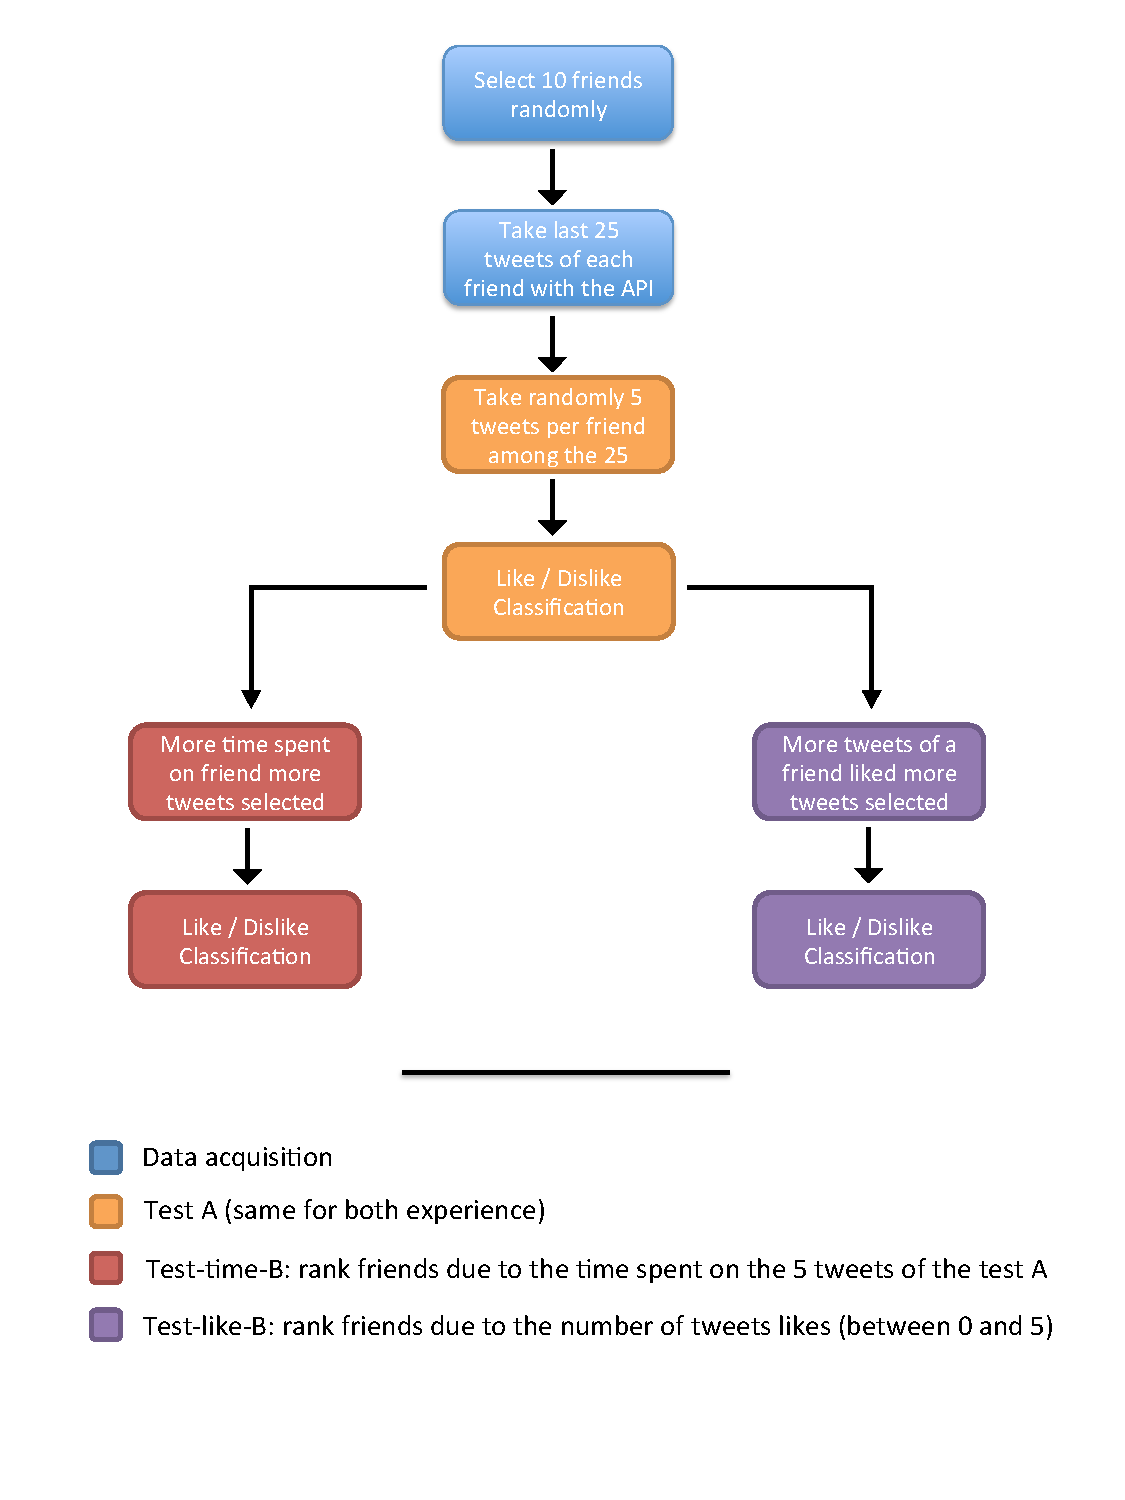
\includegraphics[width=1\columnwidth]{experiment_settings/diagram} 
\caption[Time spent of Social Media]{This clock shows the distribution of an hour online spent by US people. 16 min are on social network and forum. Source: \cite{s_clock}}
\label{fig:clock1} 
\end{figure}

\section{Experiment}

\subsection{Dataset}

As mentioned before, we decided to do a binary classification (like / dislike) of the tweets coming from the 
user's timeline. Because we use tweets from the timeline, it is assumed that users are interested by the 
content to a certain extent: they follow the writer of the tweet. In order to reduce external factors, we limit the 
timeline at a group of 10 people who the person follows, called "friends". We select 10 friends randomly who 
published at least 25 tweets. Thanks to this data, we create a simple timeline that we suppose is similar to the 
real one. When a user logs in to Twinder, we retrieve in total 250 tweets: 25 tweets coming from 10 different 
friends. In order to keep the timeline chronological, we select the most recent 25 tweets from each user. \\
In the motivation chapter, we said in the Figure 1.3 that the content of twitter is standardised with a maximum of 140 characters. However, the content can take several forms, like photos, videos, text and it starts to become a little tricky to differentiate each case. We finally consider them similar to a pure text because the majority of the tweets with images contain text. After having considered the content of the tweets, the next problem that we faced was the layout of each tweet. Indeed, after displaying only the text of the tweets, we realised that the embed layout was something important for the user. It allow him to contextualise the information and link it to twitter. (img difference of embed not). \\
The methodology of the experiment is based on the dataset assumption that we enumerated previously. The 
A/B test will be explained, it is composed of the test A (calibration) and the test B1 or B2.  

\subsection{A/B Test}

\subsubsection{A Test}






